\chapter{\MakeUppercase{Моделирование ходьбы}}
\section{Траектории движения ног}

Самым простым способом реализации ходьбы является такой, при котором робот по очереди переставляет ноги в нужном порядке, всегда имея три точки опоры. Было решено для начала взять именно эту реализацию, и немного ее модернизировать. Ноги робота будут двигаться по запрограммированной заранее траектории, перемещаясь по точкам, лежащим на этой траектории.

Движение ноги во время ходьбы было описано при помощи двух замкнутых траекторий движения точки $ A $ в двух проекциях: на плоскость $ XZ $ и $ XY $. На полученных траекториях берется множество точек, в которые управляющей программой по очереди переносится точка $A$. В качестве первого приближения для траектории в проекции на плоскость $ XZ $ был выбран эллипс (рисунок \ref{fig:traj1}), для траектории в проекции на плоскость $ XY $ выбрана линия (эллипс с нулевой малой полуосью).

\begin{figure}[h]
    \centering
    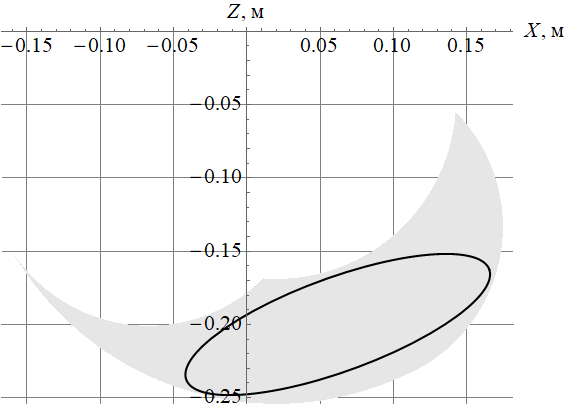
\includegraphics[scale=0.6]{chapter_walking_model/figure8.png}
    \caption{Траектория описываемая точкой $A$ в рабочей области}
    \label{fig:traj1}
\end{figure}

Точки на этой траектории достаточно легко вычислять для каждого момента времени, если замкнутая кривая описана функцией. Следует отметить, что на практике абсолютный энкодер установленный в подобранных приводах имеет <<область нечувствительности>> (рисунок \ref{fig:nonff}). Это приводит к тому, что при слишком малом расстоянии между точками, выбранными на траектории, текущая и новая конфигурации ног слабо отличаются. Это в свою очередь приводит к тому, что двигатели просто <<игнорируют>> управляющий сигнал, сообщающий о необходимости поворота на новый, слабо отличающийся угол. Упрощенная схема работы сервопривода показана на рисунке \ref{fig:upr_servo}.

\begin{figure}[h]
    \centering
    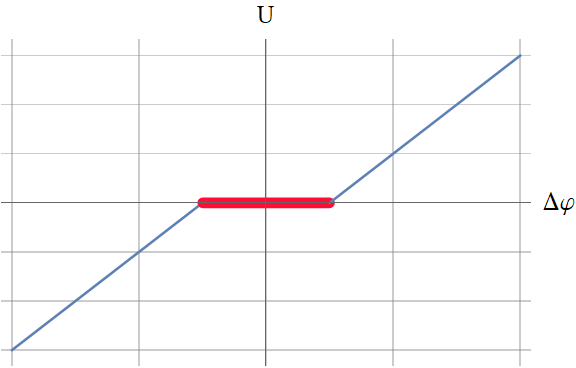
\includegraphics[scale=0.6]{chapter_walking_model/figure2.png}
    \caption{Область нечувствительности отмечена красным цветом}
    \label{fig:nonff}
\end{figure}

\begin{figure}[h]
    \centering
    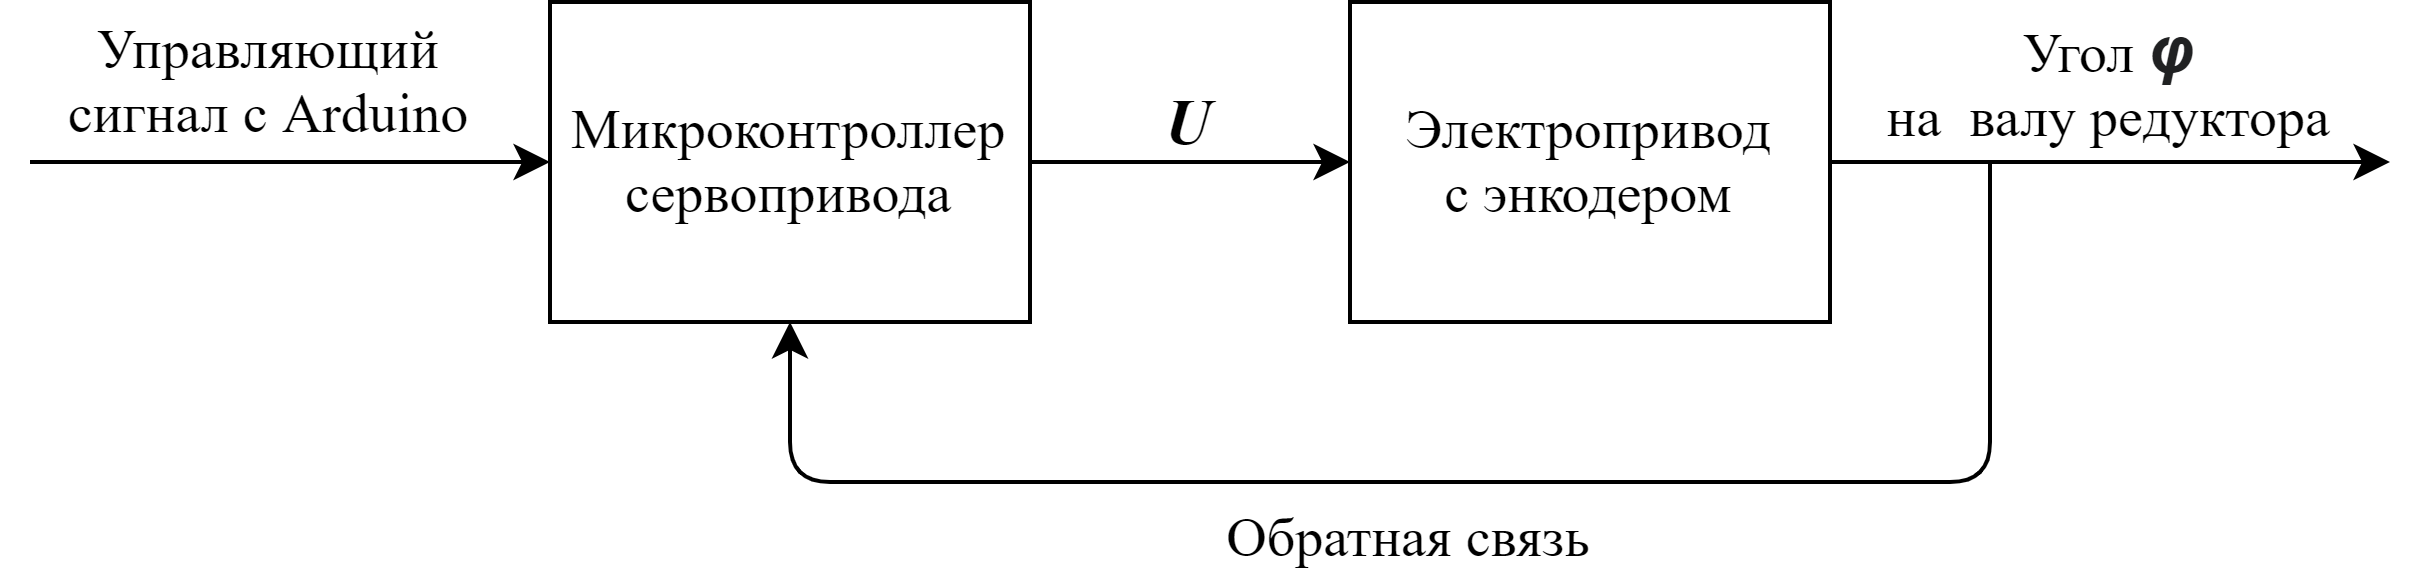
\includegraphics[width=\textwidth]{chapter_walking_model/figure1.png}
    \caption{Упрощенная схема внутренней системы управления сервопривода}
    \label{fig:upr_servo}
\end{figure}

Положим, что при смене конфигурации конечности угловая скорость сервоприводов постоянна, т.е. углы поворота меняются по линейному закону. Также учтем, что угловыми скоростями сервоприводов невозможно управлять <<извне>>, скорость задается встроенным в сервопривод микроконтроллером (рисунок \ref{fig:upr_servo}). Тогда чем меньше точек мы берем на траектории, тем менее точно конечность описывает нужную нам кривую, что наглядно показано на иллюстрации \ref{fig:traj2}, там мы берем всего четыре точки.

\begin{figure}[h]
    \centering
    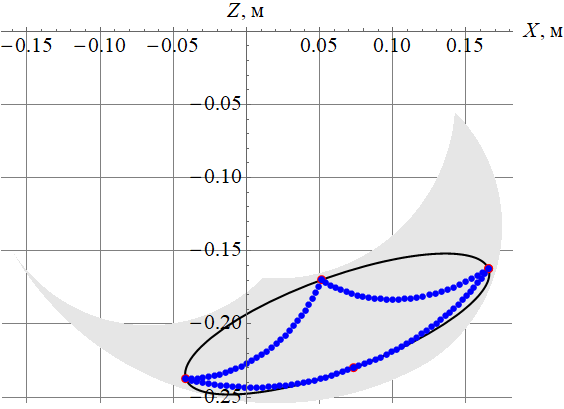
\includegraphics[scale=0.6]{chapter_walking_model/figure6.png}
    \caption{Моделирование движения между четырьмя точками траектории}
    \label{fig:traj2}
\end{figure}

\begin{figure}[h!]
    \centering
    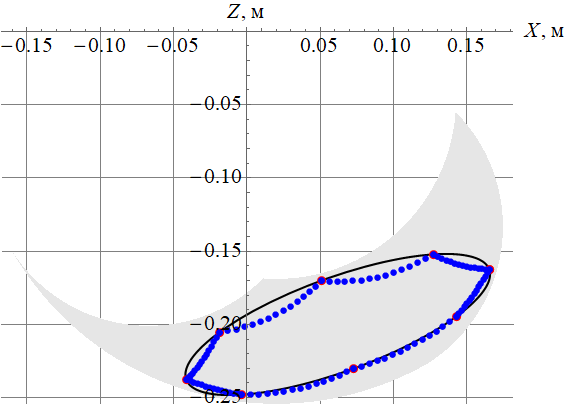
\includegraphics[scale=0.6]{chapter_walking_model/figure7.png}
    \caption{Моделирование движения мужду восьмью точками траектории}
    \label{fig:traj3}
\end{figure}

Увеличение частоты точек в два раза показало гораздо лучший результат, что можно видеть на рисунке \ref{fig:traj3}. Нижняя часть траектории описана с минимальной ошибкой. Отклонение от движения по верхней части траектории все еще сохраняется, но уже является допустимым при применении на практике.

В прототипе на данном этапе разработки применен именно этот способ движения ног.

\section{Проблема выбора оптимальной траектории}

Эллипс не является оптимальной траекторией для описания движения конечности при ходьбе. В идеале, роботам требуются более сложные траектории. Причем в них нужно вносить коррективы при любых изменениях в механике робота. Данная сложность была решена при помощи набирающих сегодня популярность искусственных нейронных сетей \cite{Singla2018}. Обученные модели сегодня могут помочь разработчикам найти оптимальный способ движения для ног робота. К сожалению, входной порог для изучения и последующего применения таких моделей очень высок, поэтому они не были применены при разработке прототипа.